%%---------------Homework Template------------------%%
%----------------------------------------------------%
\documentclass[a4paper,11pt]{article}

%---------------code settings------------------------%
\usepackage{listings}
\usepackage{xcolor}
\definecolor{mygreen}{rgb}{0,0.6,0}
\definecolor{mygray}{rgb}{0.5,0.5,0.5}
\definecolor{mymauve}{rgb}{0.58,0,0.82}

\lstset{ %
  backgroundcolor=\color{white},   % choose the background color; you must add \usepackage{color} or \usepackage{xcolor}
  basicstyle=\footnotesize,        % the size of the fonts that are used for the code
  breakatwhitespace=false,         % sets if automatic breaks should only happen at whitespace
  breaklines=true,                 % sets automatic line breaking
  captionpos=bl,                    % sets the caption-position to bottom
  commentstyle=\color{mygreen},    % comment style
  deletekeywords={...},            % if you want to delete keywords from the given language
  escapeinside={\%*}{*)},          % if you want to add LaTeX within your code
  extendedchars=true,              % lets you use non-ASCII characters; for 8-bits encodings only, does not work with UTF-8
  frame=single,                    % adds a frame around the code
  keepspaces=true,                 % keeps spaces in text, useful for keeping indentation of code (possibly needs columns=flexible)
  keywordstyle=\color{blue},       % keyword style
  %language=Python,                 % the language of the code
  morekeywords={*,...},            % if you want to add more keywords to the set
  numbers=left,                    % where to put the line-numbers; possible values are (none, left, right)
  numbersep=5pt,                   % how far the line-numbers are from the code
  numberstyle=\tiny\color{mygray}, % the style that is used for the line-numbers
  rulecolor=\color{black},         % if not set, the frame-color may be changed on line-breaks within not-black text (e.g. comments (green here))
  showspaces=false,                % show spaces everywhere adding particular underscores; it overrides 'showstringspaces'
  showstringspaces=false,          % underline spaces within strings only
  showtabs=false,                  % show tabs within strings adding particular underscores
  stepnumber=1,                    % the step between two line-numbers. If it's 1, each line will be numbered
  stringstyle=\color{orange},     % string literal style
  tabsize=2,                       % sets default tabsize to 2 spaces
  %title=myPython.py                   % show the filename of files included with \lstinputlisting; also try caption instead of title
}

%---------------------other package--------------&
\usepackage[T1]{fontenc}
\usepackage[utf8x]{inputenc}
\usepackage[english]{babel}
\usepackage{float}
\usepackage[colorlinks=true, allcolors=blue]{hyperref}
\usepackage[parfill]{parskip}
\usepackage[a4paper,top=2cm,bottom=3cm,left=1.5cm,right=1.5cm,marginparwidth=2cm]{geometry}
\usepackage{graphicx}
\usepackage{fancyhdr}
\usepackage{titlesec}
\usepackage{amsmath}
\usepackage{amssymb}
\usepackage{indentfirst}
\setlength{\headheight}{41pt}
\setlength{\parindent}{2em}


\begin{document}

%--------------fancyhead------------%
\pagestyle{fancy}
\fancyhead[R]{Classical Electrondynamics}
\fancyhead[L]{
\includegraphics[width=4.5cm]{logo/row.png}}
\fancyfoot[R]{
\includegraphics[width=3cm]{logo/spst.png}}
%---------------title---------------%
\title{\textbf{\Huge{Midterm Exam}}}

%--------------author---------------%
\author{\textit{Xinzhi Li} \\\quad\\Student ID:~~$\boldsymbol{2022211084}$\\\quad\\ \textit{School of Physics Science and Technology, ShanghaiTech University, Shanghai 201210, China}\\\quad \\ \textit{Email address}:\quad lixzh2022@shanghaitech.edu.cn}


%---------------Logo----------------%
\begin{figure*}[t]
\centering

\includegraphics[width=1\columnwidth]{logo/row.png}
\end{figure*}

%--------------maketitle--------------&
\maketitle\thispagestyle{empty}
%--------------main body--------------&
\newpage
\setcounter{page}{1}

\begin{enumerate}
    \item \textbf{Colulomb's law and Gauss theorem}
    \begin{enumerate}
        \item What is the electric field and electrostatic potential generated by a single point charge, and multiple point charges? How to define continuous charge density? What are the electric field and electrostatic potential generated by a continuous charge density distribution?
        \item Suppose a charge $q$ is in an electric field $\boldsymbol{E}(\boldsymbol{r})$, how much work is needed to move the charge from $\boldsymbol{r}_1$ to $\boldsymbol{r}_2$? What is the electrostatic potential energy for two point charges $q_1$ and $q_2$ separated by $\boldsymbol{r}$? Given a collection of point charges $\{q_i,i=1,2,3,\dots,N\}$, what is the electrostatic potential energy? Given continuous charge density distribution $\rho(\boldsymbol{r})$, what is the total potential energy? What is the energy density for the electric field $\boldsymbol{E}(\boldsymbol{r})$ generated by $\rho(\boldsymbol{r})$?
        \item Try to prove that a collection of charged particles by themselves is unstable. The charge particles cannot stay in equilibrium without other external forces. \textcolor{red}{(Hint: a particle stays in equilibrium position when its potential energy $U(x)$ satisfies $\dfrac{\partial U}{\partial x}= 0$ and $\dfrac{\partial^2 U}{\partial x^2}>0$)}
    \end{enumerate}
    \rule[0pt]{6cm}{0.05em}
    \begin{enumerate}
        \item The electric field and potential generated by a single point charge $q$ located at $\boldsymbol{r}_0$ is 
        \begin{eqnarray}
            \boldsymbol{E}(\boldsymbol{r};\boldsymbol{r}_0)=\dfrac{q}{4\pi\epsilon_0}\dfrac{\boldsymbol{r}-\boldsymbol{r}_0}{|\boldsymbol{r}-\boldsymbol{r}_0|^3},\quad\quad\quad\quad \phi(\boldsymbol{r};\boldsymbol{r}_0)=\dfrac{q}{4\pi\epsilon_0}\dfrac{1}{|\boldsymbol{r}-\boldsymbol{r}_0|}
        \end{eqnarray}

        The electric field and potential generated by multiple point charges $q_i$ located at $\boldsymbol{r}_i$ $(i=1,\dots,N)$ is 
        \begin{eqnarray}\label{eq1}
            \boldsymbol{E}(\boldsymbol{r};\boldsymbol{r}_1,\dots)=\dfrac{1}{4\pi\epsilon_0}\sum\limits^{N}_{i=1}q_i\dfrac{\boldsymbol{r}-\boldsymbol{r}_i}{|\boldsymbol{r}-\boldsymbol{r}_i|^3},\quad\quad\quad\quad \phi(\boldsymbol{r};\boldsymbol{r}_1,\dots)=\dfrac{1}{4\pi\epsilon_0}\sum\limits^{N}_{i=1}\dfrac{q_i}{|\boldsymbol{r}-\boldsymbol{r}_i|}
        \end{eqnarray}

        If the charges are so small and exist everywhere in space, they can descibed by a charge density $\rho(\boldsymbol{r})$. If there is a $\Delta q$ in a small volume $\Delta V$, then $\Delta q \approx \rho(\boldsymbol{r}) \Delta V$. Hence we can define the continuous charge density:
        \begin{equation}
            \rho(\boldsymbol{r})=\lim\limits_{\Delta V\to 0}\dfrac{\Delta q(\boldsymbol{r})}{\Delta V}
        \end{equation}
        Converting the sum over $\boldsymbol{r}$ into an integral over $\boldsymbol{r}$ through $\sum\limits_{r_i}(\dotsm)\to\int d\boldsymbol{r}'(\dotsm)$, we have the continuous form:
        \begin{eqnarray}
            \boldsymbol{E}(\boldsymbol{r})=\dfrac{1}{4\pi\epsilon_0}\int d\boldsymbol{r}'\rho(\boldsymbol{r}')\dfrac{\boldsymbol{r}-\boldsymbol{r}'}{|\boldsymbol{r}-\boldsymbol{r}'|^3},\quad\quad\quad\quad \phi(\boldsymbol{r})=\dfrac{1}{4\pi\epsilon_0}\int d\boldsymbol{r}'\dfrac{\rho(\boldsymbol{r}')}{|\boldsymbol{r}-\boldsymbol{r}'|}
        \end{eqnarray}
        \item The force acting on the charge $q$ at any point is 
        \begin{eqnarray}
            \boldsymbol{F}=q\boldsymbol{E}
        \end{eqnarray}
        Hence the work done in moving the charge from $\boldsymbol{r}_1$ to $\boldsymbol{r}_2$ is
        \begin{eqnarray}
            W=-\int_{\boldsymbol{r}_1}^{\boldsymbol{r}_2}\boldsymbol{F}\cdot d\boldsymbol{l} = -q\int_{\boldsymbol{r}_1}^{\boldsymbol{r}_2}\boldsymbol{E}\cdot d\boldsymbol{l}=q\int_{\boldsymbol{r}_1}^{\boldsymbol{r}_2}\nabla\phi\cdot d\boldsymbol{l}=q\int_{\boldsymbol{r}_1}^{\boldsymbol{r}_2}d\phi=q(\phi(\boldsymbol{r}_2)-\phi(\boldsymbol{r}_1))
        \end{eqnarray}
        
        The potential energy can be viewed that $q_2$ is brought from infinity to a point $\boldsymbol{r}_2$ where $\boldsymbol{r}=\boldsymbol{r}_2-\boldsymbol{r}_1$ in a region of electric field produced by $q_1$
        \begin{eqnarray}
            W=\dfrac{q_2}{4\pi\epsilon_0}\dfrac{q_1}{|\boldsymbol{r}_2-\boldsymbol{r}_1|}=\dfrac{1}{4\pi\epsilon_0}\dfrac{q_1q_2}{|\boldsymbol{r}|}
        \end{eqnarray}
        For a collection of point charges, the potential energy of the charge $q_i$ is 
        \begin{eqnarray}
            W_i=\dfrac{q_i}{4\pi\epsilon_0}\sum\limits_{j\neq i}^{N}\dfrac{q_j}{|\boldsymbol{r}_i-\boldsymbol{r}_j|}
        \end{eqnarray}
        The total potential energy of all the charges is 
        \begin{eqnarray}\label{eq2}
            W=\dfrac{1}{2}\times\dfrac{1}{4\pi\epsilon_0}\sum\limits_{i,j,i\neq j}^{N}\dfrac{q_iq_j}{|\boldsymbol{r}_i-\boldsymbol{r}_j|}
        \end{eqnarray}
        If we set the $i=j$ term as zero, then Eq~(\ref{eq2}) can be written as 
        \begin{eqnarray}
            W = \dfrac{1}{8\pi\epsilon_0}\sum\limits_{i,j=1}^{N}\dfrac{q_iq_j}{|\boldsymbol{r}_i-\boldsymbol{r}_j|}
        \end{eqnarray}

        Then the total continuous potential energy is 
        \begin{eqnarray}
            W=\dfrac{1}{8\pi\epsilon_0}\iint d\boldsymbol{r}d\boldsymbol{r}'\dfrac{\rho(\boldsymbol{r})\rho(\boldsymbol{r}')}{|\boldsymbol{r}-\boldsymbol{r}'|}
        \end{eqnarray}

        For a electric field $\boldsymbol{E}(\boldsymbol{r})$ generated by $\rho(\boldsymbol{r})$, we make use of Possion equation $\nabla^2\phi=-\frac{\rho}{\epsilon_0}$ to eliminate the charge density: 
        \begin{eqnarray}
            W=\dfrac{1}{2}\int d\boldsymbol{r}\rho(\boldsymbol{r})\phi(\boldsymbol{r})=-\dfrac{\epsilon_0}{2}\int d\boldsymbol{r}\phi\nabla^2\phi=\dfrac{\epsilon_0}{2}\int d\boldsymbol{r}|\nabla\phi|^2=\dfrac{\epsilon_0}{2}\int d\boldsymbol{r}|\boldsymbol{E}(\boldsymbol{r}|^2
        \end{eqnarray}
        
        Hence the energy density is 
        \begin{eqnarray}
            w(\boldsymbol{r}) = \dfrac{\epsilon_0}{2}|\boldsymbol{E}(\boldsymbol{r})|^2
        \end{eqnarray}

        \item We denote $m_i$ as the mass of the point charge, and consider the Lagrangian of the system:
        \begin{eqnarray}
            \mathcal{L}=\sum\limits_{i}\dfrac{1}{2}m_i\dot{\boldsymbol{r}}_i^2-\dfrac{1}{8\pi\epsilon_0}\sum\limits_{i,j}\dfrac{q_iq_j}{|\boldsymbol{r}_i-\boldsymbol{r}_j|}
        \end{eqnarray}
        The action is given by
        \begin{eqnarray}
            S = \int dt \mathcal{L}(\boldsymbol{r},\dot{\boldsymbol{r}})
        \end{eqnarray}

        If the system is stable, it reads $\delta S\equiv 0$ with any perturbation $\delta\boldsymbol{r}_k$
        \begin{eqnarray}
            \delta S 
            &=& \int dt\left(m_k\dot{\boldsymbol{r}}_k\delta \dot{\boldsymbol{r}}_k+\dfrac{1}{4\pi\epsilon_0}\sum\limits_{j\neq k}\dfrac{q_kq_j}{|\boldsymbol{r}_k-\boldsymbol{r}_j|^2}\delta \boldsymbol{r}_k\right)\nonumber \\
            &=& \int dt\left(-m_k\ddot{\boldsymbol{r}}_k+\dfrac{1}{4\pi\epsilon_0}\sum\limits_{j\neq k}\dfrac{q_kq_j}{|\boldsymbol{r}_k-\boldsymbol{r}_j|^2}\right)\delta \boldsymbol{r}_k
        \end{eqnarray}

        Hence we have 
        \begin{eqnarray}
            -m_k\ddot{\boldsymbol{r}}_k+\dfrac{1}{4\pi\epsilon_0}\sum\limits_{j\neq k}\dfrac{q_kq_j}{|\boldsymbol{r}_k-\boldsymbol{r}_j|^2}=0
        \end{eqnarray}

        The particle is in equilibrium, then $\ddot{\boldsymbol{r}}_k=0$, for any point charge $q_k$:
        \begin{eqnarray}\label{eq3}
            \sum\limits_{j\neq k}\dfrac{q_j}{|\boldsymbol{r}_k-\boldsymbol{r}_j|^2}=0
        \end{eqnarray}

        If $S$ is in maximum, then $\Delta S = \delta S + \dfrac{1}{2}\delta^2 S < 0$:
        \begin{eqnarray}
            \delta^2 S &=&\int dt \left(-\dfrac{1}{2\pi\epsilon_0}\sum\limits_{j\neq k}\dfrac{q_kq_j}{|\boldsymbol{r}_k-\boldsymbol{r}_j|^3}\right)(\delta \boldsymbol{r}_k)^2<0\nonumber \\
            &&\Longrightarrow \sum\limits_{j\neq k}\dfrac{q_kq_j}{|\boldsymbol{r}_k-\boldsymbol{r}_j|^3}>0
        \end{eqnarray}
        On the other hand, the energy of the system must be in minimum:
        \begin{eqnarray}
            H =T+V=\sum\limits_{i}\dfrac{1}{2}m_i\dot{\boldsymbol{r}}_i^2+\dfrac{1}{8\pi\epsilon_0}\sum\limits_{i,j}\dfrac{q_iq_j}{|\boldsymbol{r}_i-\boldsymbol{r}_j|},\quad\quad \dfrac{\partial H}{\partial\lambda}=0,\quad\quad \dfrac{\partial^2 H}{\partial\lambda^2}>0
        \end{eqnarray}
        Set the parameter $\lambda$ as $\boldsymbol{r}_k$, then we have:
        \begin{eqnarray}\label{eq4}
            \sum\limits_{j\neq k}\dfrac{q_kq_j}{|\boldsymbol{r}_k-\boldsymbol{r}_j|^3}>0
        \end{eqnarray}
        Differentiate the Eq~(\ref{eq3}) by $\boldsymbol{r}_k$, it satisfies:
        \begin{eqnarray}
            \sum\limits_{j\neq k}\dfrac{-q_j}{|\boldsymbol{r}_k-\boldsymbol{r}_j|^3}=0
        \end{eqnarray}
        which is a contradiction to Eq~(\ref{eq4}).
    \end{enumerate}
    \item \textbf{Method of images and Green's functions for typpe-I boundary conditions}
    \begin{enumerate}
        \item Consider an infinite parallel conductor plate, with a point charge $q$ at $z=b$ above the plate. The electrostatic potential on the conductor plate is zero. What is the potential above the conductor plate?
        \item Write down the Green's function $G(\boldsymbol{r},\boldsymbol{r}')$ for such a geometry.
        \item The potential on the conductor plane $z=0$ is specified as:
        \begin{equation}
            \begin{cases}
                \phi(\rho,\varphi,z=0)=V_0\quad\quad\quad\quad0\leqslant \rho\leqslant a \\
                \phi(\rho,\varphi,z=0)=0\quad\quad\quad\quad\quad \rho>a
            \end{cases}
        \end{equation}
        Please find an integral expression in cylindrical coordinates for the potential at a point $\boldsymbol{r}$ above the conductor plate.
    \end{enumerate}
    \rule[0pt]{6cm}{0.05em}
    \begin{enumerate}
        \item The image charge is under the plate at $z=-b$ with total charge $-q$
        \begin{figure}[h]
            \centering
            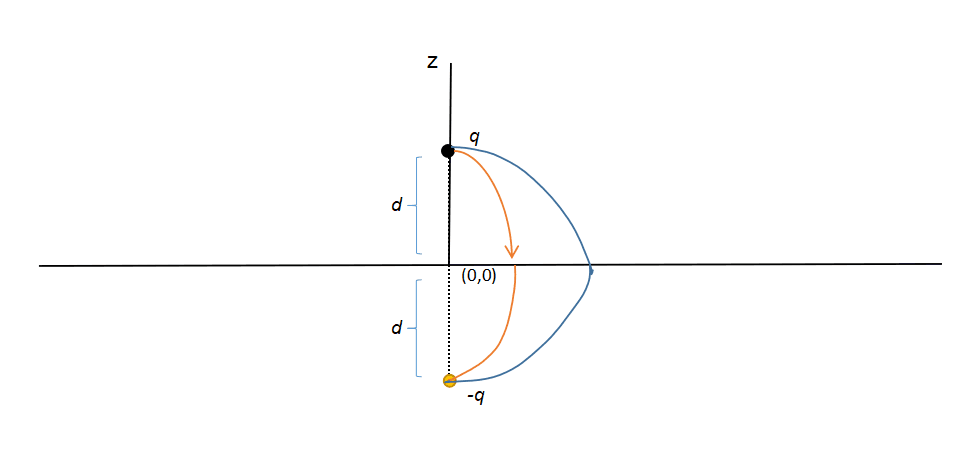
\includegraphics[width=0.5\textwidth]{fig2.png}\caption{Electrostatic potential distribution}
        \end{figure}
        
        Hence the potential distribution can be viewed as the production of the two point charge:
        \begin{equation}
            \phi(\rho,\varphi,z)=\dfrac{q}{4\pi\epsilon_0}\left[\dfrac{1}{\sqrt{(z-b)^2+\rho^2}}-\dfrac{1}{\sqrt{(z+b)^2+\rho^2}}\right]
        \end{equation}
        \item Set $\boldsymbol{r}_{+}=(\rho',\varphi',z'),\boldsymbol{r}_{-}=(\rho',\varphi',-z')$, then the Green's function $G(\boldsymbol{r},\boldsymbol{r}_{+})$ is written as 
        \begin{eqnarray}\label{eq8}
            G(\boldsymbol{r},\boldsymbol{r}_{+})
            &=&\dfrac{1}{|\boldsymbol{r}-\boldsymbol{r}_{+}|}-\dfrac{1}{|\boldsymbol{r}-\boldsymbol{r}_{-}|}\nonumber \\
            &=&\dfrac{1}{\sqrt{(\rho \cos\varphi-\rho' \cos\varphi')^2+(\rho \sin\varphi-\rho' \sin\varphi')^2+(z-z')^2}} \nonumber \\
            &&-\dfrac{1}{\sqrt{(\rho \cos\varphi-\rho' \cos\varphi')^2+(\rho \sin\varphi-\rho' \sin\varphi')^2+(z+z')^2}} 
        \end{eqnarray}
        \item The Green's function satisfies with the \textit{Dirichlet boundary conditions}, hence the formal solution is (here we use $\Omega$ to denote charge density $\rho$ in cylindrical coordinates, and $\boldsymbol{r}'$ is along z-axis):
        \begin{eqnarray}
            \phi(\boldsymbol{r})
            &=&\dfrac{1}{4\pi\epsilon_0}\int d\boldsymbol{r}_{+}\Omega(\boldsymbol{r}_{+})G(\boldsymbol{r},\boldsymbol{r}_{+})+\dfrac{1}{4\pi}\oint_S\phi(\boldsymbol{r}_{+})\dfrac{\partial G(\boldsymbol{r},\boldsymbol{r}_{+})}{\partial z'}da' \nonumber\\
            &=&\dfrac{1}{4\pi\epsilon_0}\int_{0}^{\infty} dz'\int_{0}^{2\pi} d\varphi' \int_{0}^{\infty} \rho'd\rho' \Omega(\boldsymbol{r}_{+})G(\boldsymbol{r},\boldsymbol{r}_{+})+\dfrac{1}{4\pi}\oint_{\rho'\leqslant a}V_0 \left.\dfrac{\partial G}{\partial z'}\right|_{z'=0}da' \nonumber \\
            &=&\dfrac{1}{4\pi\epsilon_0}\int_{0}^{\infty} dz'\int_{0}^{2\pi} d\varphi' \int_{0}^{\infty} \rho'd\rho' \Omega(\boldsymbol{r}_{+})\left(\dfrac{1}{|\boldsymbol{r}-\boldsymbol{r}_{+}|}-\dfrac{1}{|\boldsymbol{r}-\boldsymbol{r}_{-}|}\right)\nonumber\\
            &&+\dfrac{V_0}{2\pi}\int_{0}^{2\pi}d\varphi'\int_{0}^{a} \rho'd\rho' \left(\dfrac{z}{\left[(\rho \cos\varphi-\rho' \cos\varphi')^2+(\rho \sin\varphi-\rho' \sin\varphi')^2+z^2\right]^{\frac{3}{2}}}\right) \nonumber \\
        \end{eqnarray}
    \end{enumerate}
    \item \textbf{Laplace equation in Cartesian coordinates}
    
    Consider a hollow cuboid, $0\leqslant x\leqslant a, 0\leqslant y\leqslant b,0\leqslant z\leqslant c$, with electrostatic potential fixed on the walls of the cube:
    \begin{eqnarray}
        \begin{cases}
            \phi(0,y,z)=\phi(a,y,z)=\phi(x,0,z)=\phi(x,b,z)=0 \\
            \phi(x,y,0)=\phi(x,y,c)=V_0 \nonumber
        \end{cases}
    \end{eqnarray}
    
    \begin{enumerate}
        \item Write down Laplace equation in Cartesian coordinates, then decompose the equation into three partial differential equations with respect to three different variables $x,y,z$ respectively.
        \item Find the electrostatic potential inside the cube.
        \item What is the electric field inside the cube? What is the surface charge density on the surface $z=c$?
    \end{enumerate}
    \rule[0pt]{6cm}{0.05em}
    \begin{enumerate}
        \item The Laplace equation in Cartesian coordinates is formed as
        \begin{eqnarray}
            \left(\dfrac{\partial^2}{\partial x^2}+\dfrac{\partial^2}{\partial y^2}+\dfrac{\partial^2}{\partial z^2}\right)\phi=0
        \end{eqnarray}
        Introduce the separation of variables $\phi=X(x)Y(y)Z(z)$,
        \begin{eqnarray}
            \dfrac{1}{X}\dfrac{\partial^2}{\partial x^2}X+\dfrac{1}{Y}\dfrac{\partial^2}{\partial y^2}Y+\dfrac{1}{Z}\dfrac{\partial^2}{\partial z^2}Z=0
        \end{eqnarray}
        Then decompose the equation as
        \begin{eqnarray}\label{eq6}
            \begin{cases}
                \dfrac{1}{X}\dfrac{\partial^2}{\partial x^2}X=-\alpha^2 \\
                \quad\\
                \dfrac{1}{Y}\dfrac{\partial^2}{\partial y^2}Y=-\beta^2 \\
                \quad\\
                \dfrac{1}{Z}\dfrac{\partial^2}{\partial z^2}Z=\gamma^2 
            \end{cases}
        \end{eqnarray}
        where $\alpha^2+\beta^2=\gamma^2,\alpha,\beta,\gamma>0$
        \item Integrate the Eq~(\ref{eq6}), we obtain the general solution:
        \begin{eqnarray}
            X(x)=a_1e^{i\alpha x}+a_2e^{-i\alpha x},\quad\quad Y(y)=b_1e^{i\beta y}+b_2e^{-i\beta y}, \quad\quad Z(z)=c_1e^{\gamma z}+c_2e^{-\gamma z}
        \end{eqnarray}
        Apply the boundary conditions:
        \begin{eqnarray}
            X(x)&=&\sin(\alpha_n x) \nonumber\\
            Y(y)&=&\sin(\beta_m y) \nonumber\\
            Z(z)&=&c_1\sinh(\sqrt{\alpha_n^2+\beta_m^2} z)+c_2\cosh(\sqrt{\alpha_n^2+\beta_m^2} z) 
        \end{eqnarray}
        where
        \begin{eqnarray}
            \begin{cases}
                \alpha_n=\dfrac{n\pi}{a} \\
                \quad \\
                \beta_m=\dfrac{m\pi}{b} \\
                \quad \\
                \gamma_{nm}=\pi\sqrt{\dfrac{n^2}{a^2}+\dfrac{m^2}{b^2}}
            \end{cases}
        \end{eqnarray}
        The general solution to $\phi$:
        \begin{eqnarray}
            \phi(x,y,z)=\sum\limits_{n,m}A_{nm}\sin(\alpha_n x)\sin(\beta_m y)\sinh(\gamma_{nm} z)\nonumber \\
            +\sum\limits_{n,m}B_{nm}\sin(\alpha_n x)\sin(\beta_m y)\cosh(\gamma_{nm} z)
        \end{eqnarray}
        Make use of $\phi(x,y,0)=\phi(x,y,c)=V_0$ and orthogonality of the basis function:
        \begin{eqnarray}
            B_{nm}&=&\dfrac{4V_0}{ab}\int_{0}^{a}dx\int_{0}^{b}dy\sin(\alpha_n x)\sin(\beta_m y)\nonumber\\
            &=&\begin{cases}
                \dfrac{16V_0}{nm\pi^2}\quad\quad \textrm{$n,m$ are both odd}\\
                0\quad\quad\quad\quad\quad\quad \textrm{otherwise}
            \end{cases} \\
            A_{nm}&=&\dfrac{4V_0(1-\cosh(\gamma_{nm}c))}{ab\sinh(\gamma_{nm}c)}\int_{0}^{a}dx\int_{0}^{b}dy\sin(\alpha_n x)\sin(\beta_m y)\nonumber\\
            &=&\begin{cases}
                \dfrac{16V_0(1-\cosh(\gamma_{nm}c))}{nm\pi^2\sinh(\gamma_{nm}c)}\quad\quad \textrm{$n,m$ are both odd}\\
                0\quad\quad\quad\quad\quad\quad\quad\quad\quad\quad \textrm{otherwise}
            \end{cases} 
        \end{eqnarray}
        Hence the potential inside the cube is:
        \begin{eqnarray}
            \phi(x,y,z)=\dfrac{16V_0}{\pi^2}\sum\limits_{n}^{odd}\sum\limits_{m}^{odd}\dfrac{1}{nm}\sin(\alpha_n x)\sin(\beta_m y)\left(\dfrac{1-\cosh(\gamma_{nm}c)}{\sinh(\gamma_{nm}c)}\sinh(\gamma_{nm}z)+\cosh(\gamma_{nm}z)\right)
        \end{eqnarray}
        \item Applying $\boldsymbol{E}=-\nabla\phi$ and $\sigma=-\epsilon_0\left.\dfrac{\partial\phi}{\partial z}\right|_{z=c}$, we have
        \begin{eqnarray}
            \boldsymbol{E}(x,y,z)
            &=&-\dfrac{16V_0}{\pi^2}\sum\limits_{n}^{odd}\sum\limits_{m}^{odd}\dfrac{\alpha_n}{nm}\cos(\alpha_n x)\sin(\beta_m y)\left(\dfrac{1-\cosh(\gamma_{nm}c)}{\sinh(\gamma_{nm}c)}\sinh(\gamma_{nm}z)+\cosh(\gamma_{nm}z)\right)\hat{x} \nonumber \\
            &&-\dfrac{16V_0}{\pi^2}\sum\limits_{n}^{odd}\sum\limits_{m}^{odd}\dfrac{\beta_m}{nm}\sin(\alpha_n x)\cos(\beta_m y)\left(\dfrac{1-\cosh(\gamma_{nm}c)}{\sinh(\gamma_{nm}c)}\sinh(\gamma_{nm}z)+\cosh(\gamma_{nm}z)\right)\hat{y} \nonumber \\
            &&-\dfrac{16V_0}{\pi^2}\sum\limits_{n}^{odd}\sum\limits_{m}^{odd}\dfrac{\gamma_{nm}}{nm}\sin(\alpha_n x)\sin(\beta_m y)\left(\dfrac{1-\cosh(\gamma_{nm}c)}{\sinh(\gamma_{nm}c)}\cosh(\gamma_{nm}z)+\sinh(\gamma_{nm}z)\right)\hat{z} \nonumber \\
        \end{eqnarray}
        \begin{eqnarray}
            \sigma=-\dfrac{16\epsilon_0V_0}{\pi^2}\sum\limits_{n}^{odd}\sum\limits_{m}^{odd}\dfrac{\gamma_{nm}}{nm}\sin(\alpha_n x)\sin(\beta_m y)\left(\dfrac{1-\cosh(\gamma_{nm}c)}{\sinh(\gamma_{nm}c)}\cosh(\gamma_{nm}c)+\sinh(\gamma_{nm}c)\right) 
        \end{eqnarray}
    \end{enumerate}
    \item \textbf{Boundary-value problem in spherical coordinates}
    \begin{enumerate}
        \item A conductor sphere with radius $a$ is centered at the origin. The potential on the surface of the conductor is fixed as:
        \begin{eqnarray}
            \phi(r=a,\theta,\varphi)=V_1\cos\theta \nonumber
        \end{eqnarray}
        Suppose there is no charge outside the sphere, what is the electrostatic potential outside the sphere?
        \item There are two point charges $+q$ at $(0,0,b)$ and $-q$ at $(0,0,-b)$, both outside the sphere. The electrostatic potential on the surface of the sphere is the same as that in (a). Please find the expression for the electrostatic potential outside the sphere \textcolor{red}{(Hint:take use of Green's function method)}
    \end{enumerate}
    \rule[0pt]{6cm}{0.05em}
    \begin{enumerate}
        \item The potential satisfies with \textit{Laplace equation}, and possesses azimuthal symmetry $m=0$, the general solution is:
        \begin{eqnarray}\label{eq7}
            \phi(r,\theta)=\sum\limits_{l=0}^{\infty}\left[A_lr^l+B_lr^{-(l+1)}\right]P_l(\cos\theta)
        \end{eqnarray}
        Since there is no charge outside the sphere, the electrostatic potential at the infty is finite. Hence, all $A_l$ is zero. The coefficients $B_l$ are found by evaluating the Eq~(\ref{eq7}) on the surface of the sphere:
        \begin{eqnarray}
            V_1\cos\theta=\sum\limits_{l=0}^{\infty}\dfrac{B_l}{a^{l+1}}P_l(\cos\theta)
        \end{eqnarray}
        Using orthogonality of the Legendre series, the $B_l$ are:
        \begin{eqnarray}
            B_l&=&\dfrac{(2l+1)a^{l+1}V_1}{2}\int_{0}^{\pi}\cos\theta P_l(\cos\theta)\sin\theta d\theta \nonumber\\
            &=&\dfrac{(2l+1)a^{l+1}V_1}{2}\int_{-1}^{1}xP_l(x)dx \nonumber \\
            &=&\dfrac{(2l+1)a^{l+1}V_1}{2}\int_{-1}^{1}P_1(x)P_l(x)dx \nonumber \\
            &=&\dfrac{(2l+1)a^{l+1}V_1}{2}\dfrac{2}{3}\delta_{1,l} \nonumber \\
            &=&\begin{cases}
                a^2V_1 \quad\quad\quad\quad l=1\\
                0\quad\quad\quad\quad\quad \textrm{otherwise}
            \end{cases}
        \end{eqnarray}
        Hence, the potential outside the sphere is 
        \begin{eqnarray}
            \phi_1(r,\theta,\varphi)=V_1\dfrac{a^2}{r^2}\cos\theta\quad\quad\quad\quad (r\geqslant a)
        \end{eqnarray}
        \item According to the linear superposition principle, this problem can be decomposed as two parts:
        \begin{eqnarray}
            \begin{cases}
                \nabla^2\phi=0\\
                \left.\phi\right|_{r=a}=V_1\cos\theta
            \end{cases},
            \quad\quad\quad\quad
            \begin{cases}
                \nabla^2\phi=-\dfrac{q(\delta(\boldsymbol{r}-\boldsymbol{r}_{+})-\delta(\boldsymbol{r}-\boldsymbol{r}_{-}))}{\epsilon_0}\\
                \left.\phi\right|_{r=a}=0
            \end{cases}
        \end{eqnarray}
        where $\boldsymbol{r}_{+}=(0,0,b),\boldsymbol{r}_{-}=(0,0,-b)$.
        
        The first one is already solved. For the second one, we apply the method of images:
        \begin{eqnarray}
            \phi_2(r,\theta,\varphi)=\dfrac{1}{4\pi\epsilon_0}\Biggl[\dfrac{q}{\sqrt{r^2+b^2-2rb\cos\theta}}-\dfrac{\dfrac{a}{b}q}{\sqrt{r^2+\dfrac{a^4}{b^2}-2\dfrac{ra^2}{b}\cos\theta}} \nonumber \\
            +\dfrac{-q}{\sqrt{r^2+b^2+2rb\cos\theta}}+\dfrac{\dfrac{a}{b}q}{\sqrt{r^2+\dfrac{a^4}{b^2}+2\dfrac{ra^2}{b}\cos\theta}}\Biggr]
        \end{eqnarray}
        Hence the entire solution is:
        \begin{eqnarray}
            \phi&=&\phi_1+\phi_2\\
            &=&\dfrac{q}{4\pi\epsilon_0}\Biggl[\dfrac{1}{\sqrt{r^2+b^2-2rb\cos\theta}}-\dfrac{1}{\sqrt{r^2\dfrac{b^2}{a^2}+a^2-2rb\cos\theta}}\nonumber\\
            &&-\dfrac{1}{\sqrt{r^2+b^2+2rb\cos\theta}}+\dfrac{1}{\sqrt{r^2\dfrac{b^2}{a^2}+a^2+2rb\cos\theta}}\Biggr]+V_1\dfrac{a^2}{r^2}\cos\theta \quad\quad (r\geqslant a)
        \end{eqnarray}                            
    \end{enumerate}
    \item \textbf{Multipole expansion}
    \begin{enumerate}
        \item Given some localized charge density $\rho(\boldsymbol{r}')$, the electrostatic potential at $\boldsymbol{r}$ is:
        \begin{eqnarray}
            \phi(\boldsymbol{r})=\dfrac{1}{4\pi\epsilon_0}\int d\boldsymbol{r}'\dfrac{\rho(\boldsymbol{r}')}{|\boldsymbol{r}-\boldsymbol{r}'|}
        \end{eqnarray}
        For $r>>r'$, please derive the expressions for the contributions to $\phi(\boldsymbol{r})$ from charge monopole, dipole, and quadrupole moments in Cartesian coordinates. Write down the explicit expressions of charge monopole, dipole, and quadrupole moments in Cartesian coordinates.
        \item For $r>>r'$, please derive the expressions for the contributions to $\phi(\boldsymbol{r})$ from charge monopole, dipole, and quadrupole moments in spherical coordinates. Write down the explicit expressions of charge monopole, dipole, and quadrupole moments in spherical coordinates.
        \item Derive the relationships between the mulitipole moments in Cartesian coordinates and in spherical coordinates (for monopole, dipole, and quadrupole moments)
    \end{enumerate}
    \rule[0pt]{6cm}{0.05em}
    \begin{enumerate}
        \item Set $\boldsymbol{r}=(x,y,z),\boldsymbol{r}'=(x',y',z')$, and the Taylor expansion:
        \begin{eqnarray}
            f(\boldsymbol{r}-\boldsymbol{r}')=f(\boldsymbol{r})-\boldsymbol{r}'\cdot\nabla f(\boldsymbol{r})+\dfrac{1}{2!}(\boldsymbol{r}'\cdot\nabla)^2 f(\boldsymbol{r})+\dotsm
        \end{eqnarray}
        For $r>>r'$, $|\boldsymbol{r}-\boldsymbol{r}'|\approx r$, the potential can be expanded as 
        \begin{eqnarray}
            \phi(\boldsymbol{r})
            &=&\dfrac{1}{4\pi\epsilon_0}\int d\boldsymbol{r}'\rho(\boldsymbol{r}')\left(\dfrac{1}{r}-\boldsymbol{r}'\cdot\nabla \dfrac{1}{r}+\dfrac{1}{2!}(\boldsymbol{r}'\cdot\nabla)^2\dfrac{1}{r}+\dotsm\right) \nonumber \\
            &=&\dfrac{1}{4\pi\epsilon_0}\int d\boldsymbol{r}'\rho(\boldsymbol{r}')\left(\dfrac{1}{r}+\boldsymbol{r}'\cdot\dfrac{\boldsymbol{r}}{r^3}+\dfrac{1}{2}\sum\limits_{i,j}x'_i x'_j\dfrac{\partial^2}{\partial x_i \partial x_j}\dfrac{1}{r}+\dotsm\right)
        \end{eqnarray}
        and for $\dfrac{\partial^2}{\partial x_i\partial y_j}\dfrac{1}{r}$,
        \begin{eqnarray}
            \dfrac{\partial^2}{\partial x_i\partial y_j}\dfrac{1}{r}
            &=&\dfrac{3x_i x_j-\delta_{ij}r^2}{r^5}
        \end{eqnarray}
        hence,
        \begin{eqnarray}
            \phi(\boldsymbol{r})
            =\dfrac{1}{4\pi\epsilon_0}\int d\boldsymbol{r}'\rho(\boldsymbol{r}')\left(\dfrac{1}{r}+\boldsymbol{r}'\cdot\dfrac{\boldsymbol{r}}{r^3}+\dfrac{1}{2}\sum\limits_{i,j}(3x'_ix'_j-r'^2\delta_{ij})\dfrac{x_ix_j}{r^5}+\dotsm\right)
        \end{eqnarray}
        The expressions for charge monopole, dipole, and quadrupole moments are
        \begin{eqnarray}
            q&=&\int d\boldsymbol{r}'\rho(\boldsymbol{r}') \\
            \boldsymbol{p}&=&\int d\boldsymbol{r}'\boldsymbol{r}'\rho(\boldsymbol{r}') \\
            Q_{ij}&=&\int d\boldsymbol{r}'(3x'_ix'_j-r'^2\delta_{ij})\rho(\boldsymbol{r}') \\
            \phi(\boldsymbol{r})&=&\dfrac{1}{4\pi\epsilon_0}\left[\dfrac{q}{r}+\dfrac{\boldsymbol{p}\cdot \boldsymbol{r}}{r^3}+\dfrac{1}{2}\sum\limits_{i,j}Q_{ij}\dfrac{x_ix_j}{r^5}+\dotsm\right]
        \end{eqnarray}
        Obviously, $Q_{ij}=Q_{ji}$
        \item Make use of $\dfrac{1}{|\boldsymbol{r}-\boldsymbol{r}'|}=\sum\limits_{l=0}^{\infty}\sum\limits_{m=-l}^{l}\dfrac{4\pi}{2l+1}\dfrac{r^{l}_{<}}{r^{l+1}_{>}}Y^{*}_{l,m}(\theta',\varphi')Y_{l,m}(\theta,\varphi)$, and here $r_>=r,r_<=r'$, the potential in a spherical coordinates is written as
        \begin{eqnarray}
            \phi(\boldsymbol{r})=\dfrac{1}{4\pi\epsilon_0}\sum\limits_{l=0}^{\infty}\sum\limits_{m=-l}^{l}\dfrac{4\pi}{2l+1}q_{l,m}\dfrac{Y_{l,m}(\theta,\varphi)}{r^{l+1}}
        \end{eqnarray}
        where 
        \begin{eqnarray}
            q_{l,m}=\int d\boldsymbol{r}' Y_{l,m}^{*}(\theta',\varphi')r'^l\rho(\boldsymbol{r}')
        \end{eqnarray}
        These coefficients are called multipole moments. The monopole, dipole, quadrupole correspond with $l=0, l=1, l=2$ respectively:
        \begin{eqnarray}
            &&monopole:\quad\quad 4\pi q_{0,0}Y_{0,0}\\
            &&dipole:\quad\quad\quad \sum\limits_{m=-1}^{1}\dfrac{4\pi}{3}q_{1,m}Y_{1,m}\\
            &&quadrupole:\quad \sum\limits_{m=-2}^{2}\dfrac{4\pi}{5}q_{2,m}Y_{2,m}
        \end{eqnarray}
        \item By calculation, 
        \begin{eqnarray}
            q_{0,0}&=&\dfrac{1}{\sqrt{4\pi}}\int d\boldsymbol{r}'\rho(\boldsymbol{r}')=\dfrac{1}{\sqrt{4\pi}}q \\
            q_{1,1}&=&-\sqrt{\dfrac{3}{8\pi}}\int d\boldsymbol{r}'(x'-iy')\rho(\boldsymbol{r}')=-\sqrt{\dfrac{3}{8\pi}}(p_x-ip_y) \nonumber\\
            q_{1,0}&=&\sqrt{\dfrac{3}{4\pi}}p_z \\
            q_{1,-1}&=&\sqrt{\dfrac{3}{8\pi}}(p_x+ip_y) \nonumber\\
            q_{2,2}&=&\dfrac{1}{4}\sqrt{\dfrac{15}{2\pi}}\int d\boldsymbol{r}'(x'-iy')^2\rho(\boldsymbol{r}')=\dfrac{1}{12}\sqrt{\dfrac{15}{2\pi}}(Q_{11}-2iQ_{12}-Q_{22}) \nonumber \\
            q_{2,1}&=&-\dfrac{1}{6}\sqrt{\dfrac{15}{2\pi}}(Q_{13}-iQ_{23}) \nonumber \\
            q_{2,0}&=&\dfrac{1}{4}\sqrt{\dfrac{5}{\pi}}Q_{33}\\
            q_{2,-1}&=&\dfrac{1}{6}\sqrt{\dfrac{15}{2\pi}}(Q_{31}+iQ_{32}) \nonumber \\
            q_{2,-2}&=&\dfrac{1}{12}\sqrt{\dfrac{15}{2\pi}}(Q_{11}+2iQ_{21}-Q_{22}) \nonumber \\
        \end{eqnarray}
    \end{enumerate}
\end{enumerate}


\end{document}